\documentclass[a4paper]{article}

\usepackage{INTERSPEECH_v2}
\usepackage{multirow}
\usepackage{tipa}
\usepackage{booktabs}
\usepackage{url}
\usepackage{epstopdf}
\newcommand{\etal}{\textit{et al}.~}
% \setlength{\aboverulesep}{0pt}
% \setlength{\belowrulesep}{0pt}
\setlength{\intextsep}{10pt plus 1pt minus 3pt} %distance between floats on the top or the bottom and the text
\setlength{\textfloatsep}{12pt plus 0pt minus 4pt}%distance between two floats
\setlength{\floatsep}{12pt plus 0pt minus 2pt}%distance between floats inserted inside the page text (using h) and the text proper
% \title{Phonemic Analysis of Unsupervised Acoustic Modeling Results Using KL Divergence}
\title{On the Linguistic Relevance of Speech Units Learned by Unsupervised Acoustic Modeling}
% {Automatically Discovered Subword Units, Evaluating/Analyzing, Similarity/Effectiveness (procedure) }
% Performance of Unsupervised Acoustic Modeling
\name{Siyuan Feng, Tan Lee}
\address{
  Department of Electronic Engineering, The Chinese University of Hong Kong, Hong Kong}
\email{\{syfeng, tanlee\}@ee.cuhk.edu.hk}

\begin{document}

\maketitle
% 
\begin{abstract}
Unsupervised acoustic modeling is an important and challenging problem in spoken language technology development for low-resource languages. It aims at automatically learning a set of speech units from un-transcribed data. These learned units are expected to be related to fundamental linguistic units that constitute the concerned language. Formulated as a clustering problem, unsupervised acoustic modeling methods are often evaluated in terms of average purity or similar types of performance measures. They do not provide detailed insights on the fitness of individual learned units and the relation between them. This paper presents an investigation on the linguistic relevance of learned speech units based on Kullback-Leibler (KL) divergence. A symmetric KL divergence metric is used to measure the distance between each pair of learned unit and ground-truth phoneme of the target language. Experimental analysis on a multilingual database shows that KL divergence is consistent with purity in evaluating clustering results. The deviation between a learned unit and its closest ground-truth phoneme is comparable to the inherent variability of the phoneme. The learned speech units have a good coverage of linguistically defined phonemes. However, there are certain phonemes that can not be covered, for example, the retroflex final /er/ in Mandarin.
% This paper presents a detailed investigation on the linguistic relevance of speech units learned by unsupervised acoustic modeling. Unlike previous studies which rely mainly on simple and straightforward metrics such as purity, NMI or AP to evaluate overall performance of unsupervised acoustic modeling approaches, this paper proposes a KL divergence-based method to measure the distance between automatically learned speech units and ground-truth phonemes. Experimental results on a multilingual speech database show that automatically learned speech units by unsupervised acoustic modeling are more consistent with fundamental linguistic units, compared with labeled ground-truth phonemes.  The discrimination of learned speech units has a distinct positive correlation with the purity values among all target languages. The learned speech units have a good coverage of linguistically defined phonemes. Phonetic confusion is relieved with a larger cluster number.
\end{abstract}
\noindent\textbf{Index Terms}: unsupervised acoustic modeling, clustering, KL divergence

\section{Introduction}
Acoustic modeling (AM) refers to the task of learning and representing the statistical relation between speech signals and the basic phonetic units of a specific language. It is the core of automatic speech recognition (ASR) technology. Conventionally acoustic model training is done in a supervised manner, i.e., the training speech must be accompanied by detailed transcription at word level. As state-of-the-art ASR systems are typically built with thousand hours of speech, preparing training transcription is considered an unwelcome task and numerous approaches have been attempted to achieve semi-supervised or lightly-supervised training \cite{lamel2002lightly,fraga2011lattice,yu2010active,huang2010semi}.
% Acoustic modeling (AM) refers to the task of learning and representing the statistical relationship between speech signals and the underlying fundamental linguistic units of a specific language. It lies in the core of automatic speech recognition (ASR). Conventionally acoustic modeling is done in a supervised manner, i.e., training speech data must be accompanied by transcriptions. The acquisition of transcriptions can be time-consuming as lots of human annotation efforts are needed. 
There are also application scenarios that transcribing speech is simply not possible, for example, when no writing system and no pronunciation lexicon are available for the target language.
In recent years, there has been a growing research interest in unsupervised acoustic modeling, which assumes that only un-transcribed raw speech are available \cite{glass2012towards,jansen2013weak,lee2012nonparametric,WangLeeLeungEtAl2014,feng2016exploit}.
This is a challenging task with significant practical impact. Unsupervised acoustic modeling has been investigated mainly in applications related to low-resource languages \cite{Wang2014}, as well as in language identification \cite{li2007vector} and topic modeling \cite{harwath2013zero}. In the latest international conferences, zero-resource speech technology remains a hot topic of research \cite{versteegh2015zero}.

Given a certain amount of un-transcribed speech, unsupervised acoustic modeling can be formulated as a segmentation-clustering problem \cite{WangLeeLeungEtAl2014}. The speech signal is divided into variable-length segments, which are subsequently clustered into a limited number of groups based on acoustic similarity. Each group of segments is assigned a label that expectedly represents a basic sound unit of the language. With the labeled segments, supervised training can be applied to establish the acoustic models, which could be based on GMM-HMM \cite{steve1996large}, DNN-HMM \cite{hinton2012deep} or LSTM-RNN \cite{sak2014long}.
 % This approach, consisting of three stages, i.e. segmentation, clustering and statistical modeling, is known as Acoustic Segment Modeling (ASM) [7] – the term ASM is not popular nowadays. Perhaps we do not mention it.
% This is a challenging task, as in this scenario, transcriptions and linguistic knowledge such as subword (fundamental) unit inventories and word lexicon are unknown, thus conventional acoustic modeling approaches cannot be applied directly. With raw speech data, acoustic modeling becomes a clustering problem \cite{WangLeeLeungEtAl2014}{}, where in the ideal case each cluster is expected to match with a phoneme of the target language. Subword unit boundaries of each speech utterance are firstly discovered to combine speech frames into segments with variable length. Speech segments with similar acoustic features are then clustered, forming a series of groups. Each group represents a phoneme-like acoustic unit. The statistical distribution of each group is the corresponding acoustic model and supervised acoustic modeling techniques can be conveniently applied to establish an HMM for each cluster based on GMM-HMM or DNN-HMM structure \cite{hinton2012deep}.
 % This approach, consisting of three stages, i.e. segmentation, clustering and statistical modeling, is known as Acoustic Segment Modeling (ASM) \cite{LeeSoongJuang}.

% In practice, there are some issues which limit the performance of unsupervised acoustic modeling. 
% First, the precision of subword unit boundary detection. 
The above approach to unsupervised acoustic modeling has been investigated extensively. On unsupervised segmentation, Qiao \etal \cite{QiaoShimomuraMinematsu2008} presented a bottom-up hierarchical segmentation algorithm that exploits the spectral discontinuities at segment boundaries. Torbati \etal \cite{torbati2013speech} introduced a phoneme segmentation method based on Bayesian HMM with hierarchical Dirichlet process (HDP) priors. Estevan \etal \cite{estevan2007finding} applied the maximum-margin clustering algorithm in speech segmentation. Feng \etal \cite{feng2016exploit} proposed to use multiple language-mismatched phone recognizers to make phonetically-informed hypotheses of segment boundaries. For segment clustering, Wang \etal \cite{I3EWang} applied the spectral clustering approach with segment-level posterior features, and demonstrated superior performance as compared to vector quantization (VQ) \cite{LeeSoongJuang}, Gaussian labeling (GL) \cite{WangLeungLeeEtAl2012} and segmental GMM (SGMM) \cite{GishNg1993}.

% Con AM usually in terms of speech recognition performance, i.e., WER. This is not applicable to UAM case, because of lacking g-t transcriptions. in previous studies, XXX have been commonly used as quantitative indicators to evaluate different approaches. These metrics are simple & straightforward, suitable for overall comparisons. However, dont provide detail insights on the similarity or other properties of clusters. Purity's limitation needs to be explained by one 具体例子
The efficacy of acoustic models is evaluated typically in terms of speech recognition performance, e.g., phoneme accuracy or word error rate. This is obviously not applicable to the case of unsupervised acoustic modeling, in which there are not predefined phonemes and words. Purity \cite{I3EWang}\cite{feng2016exploit}, normalized mutual information (NMI)  \cite{I3EWang} and average precision (AP) \cite{jansen2013weak} are commonly used performance metrics for evaluating clustering algorithms. These metrics facilitate straightforward comparison of overall performance. They do not provide detailed insights on the fitness of individual clusters and the relation between the clusters. For the investigation of unsupervised acoustic modeling methods, one of the major concerns is about the linguistic relevance of the automatically learned speech units.
For example, let us consider the clustering results produced by two different clustering algorithms (or the same algorithm with different parameter settings). In the first case, the degree of overlap between an automatically learned cluster and its closest ground-truth phoneme varies greatly from one cluster to another, whereas in the second case, the degrees of overlap are equal across all clusters. Although the two sets of clustering results may give the same purity value, their linguistic implications could be very different.
In this study, we investigate the use of Kullback-Leibler (KL) divergence in the analysis of automatically learned speech units in unsupervised acoustic modeling.
KL divergence is a statistics-based distance measure that can be used to model implicit speech variation related to phonetic context, pronunciation variation, speaker characteristics, etc. It was successfully applied to ASR acoustic modeling \cite{aradilla2007acoustic}\cite{aradilla2008using}, training data selection \cite{asami2015training}, cross-lingual TTS \cite{xie2016kl} and voice conversion \cite{xie2016klvc}. 
Motivated by the successful application of KL divergence metric in measuring phonetic distortion and performing senone mapping \cite{xie2016kl}\cite{xie2016klvc}, we are interested in its effectiveness in analyzing the linguistic relevance of speech units automatically learned from an unknown language.
% The KL divergence is conceptually applicable to our task, as the similarity between automatically learned units and ground-truth phonemes can be regarded as the distance between pairs of statistical distributions.
% These metrics are simple and straightforward, suitable for overall comparisons. However, they do not provide detailed insights on the similarity or other properties of clusters. 
% The goal of unsupervised acoustic modeling is to learn fundamental subword units from raw speech, with the expectation that each automatically discovered unit (cluster) is in good accordance with one phoneme of the target language. Consider a case where two different clustering results are obtained with the same purity value. The similarities between pairs of an unsupervised subword unit and its most similar ground-truth phoneme vary a lot in the first clustering result, while keep consistent among all subword units in the second. The purity measure is unable to reveal this kind of diversity.
% Evaluation metrics of unsupervised acoustic modeling cannot be applied from convetional supervised acoustic modeling which relies mainly on word error rate (WER) or sequence error rate (SER). In the unsupervised scenario, there is no prior knowledge about the number of subword units, let alone explicit concept or the lexicon of \textit{word}. Moreover, each automatically generated subword unit is represented by its corresponding cluster index, while linguistic meaning is totally unknown. 
% Past papers mainly compared the degree to which automatically generated subword transcriptions match with ground-truth phonetic transcriptions. These metrics were solely used to evaluate overall similarity between automatically generated transcriptions and ground-truth phonetic transcriptions. However, the goal of unsupervised acoustic modeling is to learn fundamental linguistic units from raw speech, with the expectation that each automatically discovered unit (cluster) has a good correspondence with one phoneme of the target language. Most past papers claim their methods' superiority through increase on either metric(s) above, without disscussion in detail the distributions of unsupervised discovered units and their correlation between ground-truth phonemes, thus bring vagueness to the extent of linguistic acquisition. 
% In this study, we propose to present methods for a detailed analysis on clusters of unsupervised acoustic modeling results, using the Kullback-Leibler (KL) divergence as the measure.

% The KL divergence has been widely used in speech related areas. KL divergence-based HMM (KL-HMM) \cite{aradilla2007acoustic}\cite{aradilla2008using}  has been successfully utilized in specific recognition tasks, such as non-native speech \cite{razavi2014recognition}, grapheme-based speech \cite{dossgrapheme}, multilingual speech \cite{imseng2012using} and dysarthria speech \cite{kim2016dysarthric}, since KL-HMM is powerful and flexible in achieving implicit phonetic variation modeling. A state tying method based on KL divergence of DNN outputs is investigated in
% and shown its effectiveness for DNN-HMM 
% \cite{gosztolya2015building}. A training data selection strategy for improved acoustic modeling in the target-domain based on KL divergence is investigated in \cite{asami2015training}. 
% Xie \etal investigates 
% KL divergence-based phonetic distortion estimation and senone mapping is investigated with applications to cross-lingual TTS \cite{xie2016kl} and voice conversion \cite{xie2016klvc}.



% There is no prior knowledge on the number of subword units in the target language.


\section{Unsupervised Acoustic Modeling Framework}
\label{lmphnrec}
% An unsupervised acoustic modeling framework is discussed in \cite{feng2016exploit}. 
The basic framework of unsupervised acoustic modeling consists of three stages: unsupervised segmentation, segment clustering and statistical modeling \cite{feng2016exploit}.
 % The approaches developed in our previous research  are adopted here. 
Speech utterances of the target language are first divided into segments of variable length based on the hypothesized segment boundaries that are generated by a few language-mismatched phone recognizers. A spectral clustering algorithm is applied to group the speech segments into a prescribed number of clusters. Each cluster of segments is given a label. The segment labels are regarded as phone-level transcriptions, with which supervised training of acoustic models can be carried out.
The target language mentioned above is generally a low-resource language. However, in the present study, the target languages being modeled are commonly regarded as resource-rich languages. This is to facilitate the analysis of clustering results, which requires the availability of ground-truth transcription and time alignment. 
% experiments are carried out with 

% Training speech data should ideally be of real low-resource languages. However, the current study is focused on investigating the linguistic relevance of speech units learned from raw speech. For experimental purpose, ground-truth knowledge of transcriptions and phoneme definitions are needed for performance evaluation. The resources are generally not available for low-resource languages. To this end, we instead use resource-rich languages, while transcriptions and lexicon are used only for experimental analysis.

% Each cluster can then be used to train an acoustic model in a supervised manner. 
The features extracted for segment clustering are segment-level posteriors. They are derived from the frame-level posteriors produced by the language-mismatched phone recognizers. Let $\bm{x_t}$ be the acoustic observation of the $t$-th frame. The frame-level posterior feature vector is defined as, 
% The phoneme posterior space in this paper is constructed by senones (phonemes) of the neural network (NN)-based phoneme recognizer for a language different from the target language, with the assumption that no linguistic knowledge of the target language is available.
% By using a language-mismatched phoneme recognizer, we are meant to follow the unsupervised scenario, in which the target language is unknown. 
% Let $\{\bm{x_1}, \bm{x_2}, \ldots, \bm{x_T}\}$ denote acoustic features (e.g., MFCCs) of $T$ speech frames. Outputs of the phoneme recognizer are frame posterior probability vectors as shown below:
\begin{equation}  
 \bm{q_t} =  \left[  
  \begin{array}{c}  
          p(c_1 \vert \bm{x_t}) \\  
          % p(c_2 \vert \bm{x_t}) \\
          \vdots \\  
          p(c_m \vert \bm{x_t}) \\
          \vdots \\
          p(c_M \vert \bm{x_t}) \\
 \end{array}  
 \right], t=1, 2, \ldots, T, 
\end{equation}
where $\{c_1, c_2, \ldots, c_M\}$ denote $M$ phoneme classes covered by multiple recognizers, $p(c_m \vert \bm{x_t})$ is the posterior probability of $c_m$ given $\bm{x_t}$. By taking the average of frame-level posterior vectors in a hypothesized segment, the segment-level posterior vector is obtained as,
\begin{equation}
\bm{\hat{x}_k} = \frac{1}{e_k - b_k +1} \sum\limits_{t = b_k}^{e_k}\bm{\hat{q}_t}, k=1, 2,\ldots, K, 
\end{equation}
where $K$ is the number of segments, $b_k$ and $e_k$ denote the beginning and the end of the $k$-th segment.
% Each segment is represented by a posterior feature. 
By segment clustering, the hypothesized segments are grouped into a prescribed number of clusters.
Each cluster corresponds to an automatically learned speech unit, which is represented by the probability distribution of frame-level posterior features. Similarly, if the ground-truth time alignments of all phonemes are given, each phoneme can be represented by the probability distribution of frame-level posterior features.
% The distribution of frame-level posterior features belonging to each cluster is a statistical representation for one automatically learned speech unit. 
% On the other hand, given reference time-aligned transcriptions for target speech data, each labeled ground-truth phoneme is represented by the probability distribution of its frame posterior features.

Each language-mismatched phone recognizer serves as a nonlinear mapping between the acoustic space and the phonetic space. Through this mapping, irrelevant variations of acoustic features, e.g., speaker, gender, channel and environmental noise, are suppressed and/or normalized. 
It is assumed, with good reasons, that the phonetic spaces of different languages are substantially overlapped, since they are all based on the same mechanism of speech production. Compared with acoustic features, posterior features are more reliable in reflecting inherent phonetic characteristics of the target language.
% Here the assumption that sounds produced in different spoken languages have significant overlap.

% In the phoneme posterior space, the coordinates are defined as phoneme posteriors, which is a probabilistic representation in the phoneme posterior space. Therefore, measuring the difference between probability distributions can be realized by measuring the distance between posterior probability vectors. 

% \begin{figure*}[!tbp]
% \centering
%   % \includegraphics[width = 0.8\textwidth]{framework.pdf}
%   % \caption{Acoustic Segment Modeling framework used in this work}
%   \label{framework}
% \end{figure*}

% \section{KL Divergence-Based Distance}
\section{Distance Between Speech Classes and Ground-Truth Phonemes}
We propose a KL divergence-based method to measure the distance between each pair of automatically learned speech unit and ground-truth phoneme in the target language.
The KL divergence, also called information divergence, or relative entropy, is a measure of the difference between two probability distributions \cite{kullback1951information}. For discrete probability distributions $P$ and $Q$, the KL divergence is defined as \cite{mackay2003information},
\begin{equation}
\label{kld_d}
  D_{KL} (P \vert \vert Q) = \sum\limits_{i} P(i) \log \frac{P(i)}{Q(i)}.
\end{equation}
Equation (\ref{kld_d}) gives a non-symmetric measure. In this paper the following symmetric discrete form of KL divergence is adopted,
\begin{align}
D_{KL} (P, Q) &= D_{KL} (P \vert \vert Q) + D_{KL} (Q \vert \vert P)\\
  &= \sum_{i} (P(i)-Q(i))\cdot \log \frac{P(i)}{Q(i)}.
\end{align}
The symmetric KL divergence is used to measure the distance between posterior feature distributions between each pair of automatically learned speech unit and ground-truth phoneme.
% \section{Distance Between Speech Classes in Phoneme Posterior Space}
% Usually after Acoustic Segment Modeling, each learned unit is assigned by a group of frames belonging to that cluster \cite{feng2016exploit}. 
% Without violation of the unsupervised scenario, time-aligned transcriptions are removed during training stage, while in results evaluation phase, they are included for reference.
% Although in the unsupervised scenario, no resource other than raw speech is assumed available. In practice, phonetic transcriptions are removed during training procedure and at evaluation stage, they are used for reference. 
% \subsection{Distance Between Learned Speech Units and Ground-Truth Phonemes}

Let $\{g_1, g_2, \ldots, g_K\}$ denote $K$ ground-truth phonemes. $\bm{v_{1}}, \bm{v_{2}}, \ldots, \bm{v_{L_k}}$ are the posterior probability vectors of $L_k$ frames that are labeled as phoneme $g_k$ according to ground-truth transcription. $\{\bm{v_{1}}, \bm{v_{2}}, \ldots, \bm{v_{L_k}}\}$ is a subset of $\{\bm{q_1}, \bm{q_2}, \ldots, \bm{q_T}\}$.
The centroid of $g_k$ is computed as,
\begin{equation}
  \bm{\overline{v^{k}}} = \frac{\sum\limits_{i=1}^{L_k}\bm{v_{i}}}{L_k}.
  \label{centroid vector of g_k}
\end{equation}
$\bm{\overline{v^k}}$ is treated as the representative of $g_k$ in the phonetic space. 
Let $\{u_1, u_2, \ldots, u_R\}$ denote $R$ automatically learned speech units, $\{\bm{\mu_{1}}, \bm{\mu_{2}}, \ldots, \bm{\mu_{N_r}}\} \subset \{  \bm{q_1}, \bm{q_2}, \ldots, \bm{q_T} \}$ are the posterior probability vectors of frames assigned to $u_r$ ($r=1, 2, \ldots, R$). The distance between $u_r$ and $g_k$ is defined as,
% the average of the KL divergence between $\bm{\overline{v^k}}$ and frame posterior vectors $\bm{\mu_{j}}$ over $N_r$($j = 1, 2, \ldots, N_r$):
\begin{align}
D (u_r, g_k) &= \frac{\sum\limits_{j=1}^{N_r} D_{KL} (\bm{\mu_{j}}, \bm{\overline{v^k}} ) }{N_r}  \label{distancedef1}\\
% \label{equation1}
 &= \frac{\sum\limits_{j=1}^{N_r}  \sum\limits_{m=1}^{M} (\mu_{j} (m) -  {\overline{v^k}} (m)  )\cdot \log \frac{\mu_{j} (m)}{{\overline{v^k}}(m)} }{N_r}. \label{distancedef2}
\end{align}
Here, the distortion between two acoustic models $u_r$ and $g_k$ is measured by the KL divergence-based distance between posterior features in the phonetic space.

For each learned speech unit $u_r$, let $g_{k^{*}} (u_r)$ denote the closest ground-truth phoneme, where
\begin{equation}
k^* = \mathop{\arg\min}_{k} D(u_r, g_k). \label{optimal k}
\end{equation}
Let $g_{k^*} (u_r)$ be abbreviated as $g^* (u_r)$. The distance between $u_r$ and $g^* (u_r)$, denoted as $D^* (u_r)$, is computed by
% Here $g_{k^*} (u_r)$ is denoted as $g^* (u_r)$ for brevity without causing any confusion. For Their distance $D^* (u_r)$:
% \begin{align}
% D^* (u_r) &= \mathop{\min}_{k} D(u_r, g_k) \label{mindistance1}
% \\
% &= D(u_r, g^* (u_r))
% \label{mindistance2}
% \end{align}

\begin{equation}
D^* (u_r) = D(u_r, g^* (u_r)). \label{mindistance1}
\end{equation}
Subsequently, the distance between $u_r$ and the second closest phoneme $g_{k^{**}} (u_r)$ (abbreviated as $g^{**} (u_r)$) is calculated by
\begin{equation}
 k^{**} = \mathop{\arg\min}_{k \neq k^*} D(u_r, g_k). \label{suboptk}
\end{equation}
 The distance $D (u_r, g^{**} (u_r))$ is denoted as $D^{**} (u_r)$.
 % , where, 
% \begin{equation}
 % D^{**} (u_r) = \mathop{\min }_{k \neq k^*} D(u_r, g_k) \label{suboptdistance}
% \end{equation}
 The discrimination capability of the cluster $u_r$ can be measured by
 % $D^{*} (u_r)$ and $D^{**} (u_r)$ is named \textit{KL divergence gap}, denoted as $\Delta D^*(u_r)$,
\begin{equation}
\Delta D^{*} (u_r) = \left| D^{**} (u_r) - D^{*} (u_r) \right|. \label{divergencegap}
\end{equation}
 A small value of $D^* (u_r)$ means that the automatically learned unit matches well with one of the ground-truth phonemes. Meanwhile, a large value of $\Delta D^* (u_r)$ indicates that $g^* (u_r)$ is discriminatively mapped to $u_r$. 
% While target language and recognizer's language have their own distinctive linguistic properties, 

% These features are put into a NN-based phoneme recognizer and corresponding outputs are denoted as

% A NN-based phoneme recognizer is functioned as a nonlinear mapping between acoustic space and senone posterior space.
\label{dist_un_phn}
% \subsection{Phoneme Inner Variation}

The distance measure can be further extended to evaluating inherent variability of each ground-truth phoneme. For the phoneme $g_k$, the inherent variability is obtained as $\widetilde{D}(g_k)$,
\begin{align}
 \widetilde{D}(g_k)&= \frac{\sum\limits_{j=1}^{L_k} D_{KL} (\bm{v_{j}}, \bm{\overline{v^k}} ) }{L_k}.  \label{distanceinner}
 % \\ &=\frac{\sum\limits_{j=1}^{L_k} D_{KL} (\bm{v_{j}}, \frac{\sum\limits_{i=1}^{L_k}\bm{v_{i}}}{L_k}) }{L_k}
\end{align}
A small value of $\widetilde{D}(g_k)$ indicates that the acoustic-phonetic properties of $g_k$ are highly consistent in the training speech. It must be noted that $D^* (u_r)$ computed for learned speech units and $\widetilde {D}(g_{k^*})$ for ground-truth phonemes are comparable, as both of them measure the deviation from a class of posterior feature vectors to the centroid of the same phoneme class $g_{k^*}$, in the same phonetic space. $\widetilde{D} (g_{k^*})$ is calculated from ground-truth transcription, and independent of the clustering results. Therefore $\widetilde{D} (g_{k^*})$ could be a good reference for $D^* (u_r)$.

The KL divergence metric in this paper is not only applicable to posterior features extracted from phone recognizers, but also to conventional spectral features like MFCCs, or neural network bottle-neck features (BNFs). 
% $\sum\limits _{i}^{b}$
\section{Experimental Design}

An experimental system of unsupervised acoustic modeling is established to generate automatically learned speech units from un-transcribed speech data of a target language. The symmetric KL divergence is used to analyze the linguistic relevance of these learned units with respect to the ground-truth phonemes.
\subsection{Databases}
Spontaneous story-telling speech from the OGI Multi-language Telephone Speech Corpus (OGI-MTS) \cite{MuthusamyColeOshika1992} are used in our experiments. There are five target languages involved: German (GE), Hindi (HI), Japanese (JA), Mandarin (MA) and Spanish (SP). The corpus provides manual time alignment at phoneme level. The amount of speech data (in hours) and the number of labeled phonemes (including silence) for each language are summarized as in Table \ref{datasize}.
% Experiments of unsupervised acoustic modeling are carried out with the OGI Multi-language Telephone Speech (OGI-MTS) Corpus \cite{MuthusamyColeOshika1992}. The spontaneous story-telling speech for German (GE), Hindi (HI), Japanese (JA), Mandarin (MA) and Spanish (SP) is used. In addition to the audio signals, the database provides manual time alignment at phoneme level. The amount of data (in hours) and the number of labeled phonemes (including a silence label) for each language is summarized in Table \ref{datasize}.

\begin{table}[htbp]
\renewcommand\arraystretch{1}
\centering
\caption{Multi-lingual speech data from the OGI-MTS corpus}
\resizebox{0.8 \linewidth}{!}{%
\begin{tabular}{rccccc}      
% \hline      
\toprule
Language:  &GE&HI&JA&MA & SP \\
% \hline
\midrule
Data size:  & $1.31$ & $0.95$ & $0.86$ & $0.57$ & $1.46$\\

$\#$ Phonemes: &$43$& $46$&$ 29$& $44$& $38$\\
% \hline
\bottomrule
\end{tabular}%
}
\label{datasize}
\end{table}


% \subsection{Phoneme Recognizers}
\subsection{Automatically Learned Speech Units}
\label{purity results}
% \subsubsection{d}{}
Implementation of the unsupervised acoustic modeling framework in this work is based on approaches in \cite{feng2016exploit}. Four language-mismatched phone recognizers are used as feature extractors to generate frame-level posterior features. They are Czech (CZ), Hungarian (HU), Russian (RU) and Cantonese (CT) phone recognizers. The CZ, HU and RU recognizers were developed and made publicly available by Brno University of Technology \cite{schwarz2009phoneme}. The number of phonemes being modeled are $45$, $61$ and $52$, respectively. The CT recognizer is trained with the CUSENT database, which was developed by The Chinese University of Hong Kong to support general ASR applications \cite{LeeLoChingEtAl2002}. The number of phonemes in the CT recognizer is $73$. 

% is included in this study, in view of providing a wider coverage of phonetic space. The four recognizers act as feature extractors to generate frame-level posterior features. The CZ, HU and RU recognizers were developed and made publicly available by the Brno University of Technology \cite{schwarz2009phoneme}. The number of phonemes being modeled are 45, 61 and 52, respectively. The CT phone recognizer was trained with the CUSENT database, which was developed by the Chinese University of Hong Kong to support general ASR applications \cite{LeeLoChingEtAl2002}. The number of phonemes in the CT recognizer is 73. 

A spectral clustering algorithm is applied to cluster the segments into $R$ clusters, where $R = 50, 60, 70, 80, 90$ in our experiments. Each of these clusters is assigned a label, which denotes one of the learned speech units.  By assigning cluster labels to all segments in an input utterance, we essentially obtain a time-aligned transcription for the utterance.

% The purity is used to measure 
The similarity between automatically learned transcription and ground-truth transcription can be quantified by the purity measure. 
% The learned transcriptions are compared with ground-truth transcriptions via purity.
% Assume the posterior probability vectors of the $t$-th frame generated by CZ, HU, RU and CT phoneme recognizers are denoted as $\bm{q^{cz}_{t}}$, $\bm{q^{hu}_{t}}$, $\bm{q^{ru}_{t}}$ and $\bm{q^{ct}_{t}}$. A larger-scale frame posterior vector is constructed as the concatenation of the above four vectors as,
% \begin{equation}
% \bm{\hat{q}_t} = \left[  
%   \begin{array}{c}  
%           % p(c_1 \vert \bm{x_t}) \\  
%           \bm{q^{cz}_{t}} \\
%           \bm{q^{hu}_{t}} \\
%           \bm{q^{ru}_{t}} \\
%           \bm{q^{ct}_{t}} \\
%  \end{array}  
%  \right]
% \end{equation}
% By taking average of frame-level posterior vectors based on automatically detected segment boundaries, segment-level posterior vectors are obtained as,
% \begin{equation}
% \bm{\hat{x}_k} = \frac{1}{e_k - b_k +1} \sum\limits_{t = b_k}^{e_k}\bm{\hat{q}_t}, k=1,2,\ldots, K
% \end{equation}
% where $K$ is the number of segments of the entire training data, $b_k$ and $e_k$ are starting and ending positions of the $k$-th segment. These positions are obtained from fusion of segmentation results from CT, HU, RU and CT recognizers using the algorithm in \cite{feng2016exploit}. The segment-level posterior vectors $\{\bm{\hat{x}_1}, \bm{\hat{x}_2}, \ldots, \bm{\hat{x}_K}\}$ are clustered into groups of a pre-defined number $R$, from which each speech segment is assigned with a cluster index.
% Purity is used in this part as the measure of overall degree to which clusters are in accordance with ground-truth labels.
Let $R^{\prime}$ be the number of ground-truth phonemes, $n_{r, r^{\prime}}$ denote the number of frames assigned to the $r$-th cluster and labeled as the $r^{\prime}$-th ground-truth phoneme. The overall purity is defined as,
\begin{equation}
\mathrm{purity} = \frac{\sum\limits_{r=1}^{R}\max\limits_{r^{\prime} \in \{1,2,...,R^{\prime}\}}n_{r, r^{\prime}}}{\sum\limits_{r=1}^{R} \sum\limits_{r^{\prime}=1}^{R^{\prime}}n_{r, r^{\prime}}}.
\end{equation}
The purity values for each target language with $R$ ranging from $50$ to $90$ are shown as in Table \ref{purity as setups}.
\begin{table}[htbp]
  \centering
    \caption{Purity for the five target languages}
    \renewcommand\arraystretch{1}
    \resizebox{1 \linewidth}{!}{%
  \begin{tabular}{ccccccc}
  %\hline
  % \hline
  \toprule
    & $R=50$ & $R= 60$ & $R=70$ & $R=80$ & $R=90$ & Average\\
  % \hline
  \midrule
  %\hline
  GE &$0.428$ & $0.433$ & $0.439$ & $0.437$& $0.437$&$0.43$ \\
  % \hline
  HI &$0.494$ & $0.499$ & $0.492$& $0.489$& $0.485 $&$0.49$\\
  % \hline
  JA &$0.545$ & $0.556$ & $0.554$& $0.543$& $0.540 $&$0.55$\\
  % \hline
  MA &$0.414$ & $0.425$ & $0.434$& $0.426$& $0.426 $&$0.42$\\
  % \hline
  SP &$0.556$ & $0.586$ & $0.576$& $0.568$& $0.573 $&$0.57$\\
  % \hline
  \bottomrule
  % \hline
  % Average &  \\
  % \hline
  %\multirow{2}{*}{Multi-Row} & \multicolumn{2}{|c|}{Multi-Column} & \multicolumn{2}{|c|}{\multirow{2}{*}{Multi-Row and Col}} \\
  %\cline{2-3}
  %& column-1 & column-2 & \multicolumn{2}{|c|}{}\\
  %\hline
  \end{tabular}%
  }
  \label{purity as setups}
\end{table}
% \subsection{Purity Measure}
\section{Results and Analysis}
The relation between automatically learned speech units and ground-truth phonemes is analyzed for each target language, based on the clustering results and the ground-truth time alignment provided in the corpus. For each learned speech unit $u_r$, Equations (\ref{distancedef1}), (\ref{optimal k}) and (\ref{mindistance1}) are used to determine its closest ground-truth phoneme $g^* (u_r)$ and the distance $D^* (u_r)$ between them. Equation (\ref{suboptk}) is used to determine the second closest ground-truth phoneme $g^{**} (u_r)$ and the distance $D^{**} (u_r)$. For each ground-truth phoneme $g_k$, Equation (\ref{distanceinner}) is used to calculate the inherent variability $\widetilde{D}(g_k)$. 
The average values of $D^* (u_r)$, $D^{**} (u_r)$ and $\widetilde{D} (g_k)$ are summarized in Table \ref{KLD-subKLD-innerKLD}.
\begin{table}[htbp]
  \centering
    \caption{$\overline{D^* (u_r)}/\overline{D^{** }(u_r)}$ and $\overline{\widetilde{D}(g_k)}$}
    \renewcommand\arraystretch{1.0}
    \resizebox{\linewidth}{!}{%
  \begin{tabular}{ccccccc}
  %\hline
  % \hline
  \toprule
    & $R=50$ & $R= 60$ & $R=70$ & $R=80$ & $R=90$ &$\overline{\widetilde{D}(g_k)}$\\
  % \hline
  \midrule
  %\hline
  GE &$27.4/30.1$ & $27.3/30.0$ & $27.3/30.1$ & $27.5/30.3$& $27.4/30.3$ &$27.8$\\
  % \hline
  HI &$27.6/31.5$ & $27.6/31.6$ & $27.8/31.7$& $28.0/31.7$& $28.1/31.8$&$28.5$\\
  % \hline
  JA &$28.5/34.1$ & $28.0/33.2$ & $28.1/33.2$& $28.3/33.4$& $28.6/34.1$&$27.9$\\
  % \hline
  MA &$29.3/31.2$ & $29.3/31.5$ & $29.0/31.0$& $29.5/31.6$& $29.4/31.3$&$29.1$\\
  % \hline
  SP &$28.5/31.9$ & $27.8/32.2$ & $27.9/32.3$& $28.1/32.5$& $28.0/32.4$&$28.0$\\
  % \hline
  \bottomrule
  % \hline
  % Average &  \\
  % \hline
  %\multirow{2}{*}{Multi-Row} & \multicolumn{2}{|c|}{Multi-Column} & \multicolumn{2}{|c|}{\multirow{2}{*}{Multi-Row and Col}} \\
  %\cline{2-3}
  %& column-1 & column-2 & \multicolumn{2}{|c|}{}\\
  %\hline
  \end{tabular}%
  }
  \label{KLD-subKLD-innerKLD}
\end{table}
As seen from Table \ref{purity as setups} \& \ref{KLD-subKLD-innerKLD}, both the purity values and the average KL divergence are not sensitive to the cluster $R$.

Figure \ref{dkld-purity} compares the average values of $\Delta D^* (u_r)$ and the purity values for the five target languages.
% $\overline{\Delta D^* (u_r)}$ by Equation (\ref{divergencegap}), 
\begin{figure}[htbp]
 \centering
 \includegraphics[width = 0.486 \linewidth]{kldgapfixed.eps}
 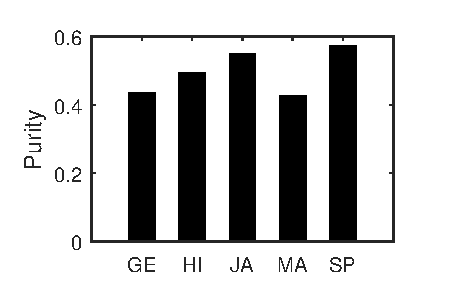
\includegraphics[width = 0.49 \linewidth]{purityfixed.eps}
 \caption{Average values of $\Delta D^* (u_r)$ and purity values}
  \label{dkld-purity}
 \end{figure}  
From Table \ref{KLD-subKLD-innerKLD} and Figure \ref{dkld-purity}, the following observations are made:
\begin{itemize}
\item[(a)] $\overline{D^* (u_r)}$ is smaller than or approximately equal to $\overline{\widetilde{D} (g_k)}$ for all target languages. In other words, the deviation between an automatically learned speech unit and its closest ground-truth phoneme is comparable to, if not smaller than, the inherent variability of the phoneme itself. In fact, the ground-truth phonemes are labeled based on auditory perception of linguistic experts, whereas the learning of speech units, as well as the proposed KL divergence metric, is totally data-driven.
% , which makes this finding explainable.
\item[(b)] The average values of $\Delta D^* (u_r)$ for different languages have the same trend as the purity values. This observation is consistent with our expectation, as a larger $\Delta D^* (u_r)$ implies that the automatically learned speech unit is mapped to its closest ground-truth phoneme with a higher confidence, thus naturally leads to a higher purity. 
\end{itemize}



We are interested to understand more about the phonetic coverage of automatically learned speech units.  
Each learned unit corresponds to one best-matching ground-truth phoneme based on Equation (\ref{optimal k}).
If a ground-truth phoneme fails to be selected as the best-matching phoneme for any of the learned units, it is regarded as not being covered. Table \ref{No. phonemes faild to map} shows the counts of uncovered vowels and consonants for each target language for $R=90$.
% To explore the phonetic coverage of the automatically learned speech units, the number of labeled ground-truth phonemes which fail to be the closest phoneme of any learned speech unit is counted. We choose $R=90$ for the example. Categorized into vowels and consonants, the numbers are summarized in Table \ref{No. phonemes faild to map}. 
\begin{table}[htbp]
  \centering
    \caption{Uncovered/total No. vowels and consonants ($R=90$)}
    \renewcommand\arraystretch{1}
    \resizebox{0.75 \linewidth}{!}{%
  \begin{tabular}{rccccc}
  %\hline
  % \hline
  \toprule
    & GE & HI & JA & MA & SP\\
  % \hline
  \midrule
  %\hline
  % \hline
  Vowels &$1/18$ & $0/13$ & $0/7$ & $2/17$& $1/11$ \\
  % \hline
  Consonants &$1/24$ & $3/32$ & $0/21$& $4/26$& $1/27 $\\
  % \hline
  \bottomrule
  \end{tabular}%
  }
  \label{No. phonemes faild to map}
\end{table}
It can be seen that most of the linguistically-defined phonemes could be covered in the process of unsupervised acoustic modeling. Particularly in the case of Japanese, all phonemes are covered. However, there are quite a few phonemes of Mandarin that are not covered by the learned units. The missing vowels and consonants are \{/aa/ (/\textipa{a}/)\footnote{Phoneme label /aa/ is used in OGI-MTS database \cite{MuthusamyColeOshika1992}, the corresponding IPA transcription is /\textipa{a}/. Similarly hereinafter.}, /er/ (/\textrhookschwa/)\} and \{/kh/ (/\textipa{k\super{h}}/), /ph/ (/\textipa{p\super{h}}/), /r/ (/\textipa{\:R}/), /tH/ (/\textipa{t\super{h}}/)\}, respectively.
% It can be seen that automatically learned units by unsupervised acoustic learning have a good coverage of linguistically defined phonemes, especially in Japanese, where all the phonemes are covered. 
% Note that Japanese has much less phonemes than other target languages, thus learning linguistically-like speech units is expected to be easier. 
% For Mandarin, however, quite a few ground-truth phonemes cannot be covered by learned units. The missing vowels and consonants are \{/aa/ (/\textipa{a}/)\footnote{Phoneme label /aa/ is used in OGI-MTS database \cite{MuthusamyColeOshika1992}, the corresponding IPA transcription is /\textipa{a}/. Similarly hereinafter.}, /er/ (/\textrhookschwa/)\} and \{/kh/ (/\textipa{k\super{h}}/), /ph/ (/\textipa{p\super{h}}/), /r/ (/\textipa{\:R}/), /tH/ (/\textipa{t\super{h}}/)\}, respectively. 
It is interesting to see that the majority of missing consonants are unvoiced plosives. These consonants have strong transitory characteristics, i.e., rapidly changing spectral properties. 
In the segmentation process of unsupervised acoustic modeling, it is assumed that individual frames in the same segment have similar spectral properties. This assumption is not valid for transitory phonemes.
Similarly, the missing vowel /er/, known as Erhuayin in Mandarin, also has transitory properties.
% , which may be the reason for not covered by learned speech units. 
This inspires us to investigate alternative features and segment representation which could capture trajectory characteristics of phonemes. 

It is not expected that the vowel /aa/ is missed. Although /aa/ is not selected as the closest phoneme to any of the learned units, it is actually identified as the second closest phoneme to two different learned units. These two units are corresponded to /ae/ (/\textipa{a}/) and /aw/ (/\textipa{au}/) according to the KL divergence. In the transcription of Mandarin speech in OGI-MTS database, /aa/ is used to label the vowel nucleus in the Pinyin Finals /a/ and /ang/, while /ae/ is used to label the vowel nucleus in the Pinyin Final /an/ \cite{wiki-nourl:xxx}. The two vowel nuclei are actually very similar in articulation. 
% \footnotetext{Labels used in Pinyin Table \cite{wiki:xxx}}
% and /ae/ are used to label the vowel nuclei in the Finals /ang/ and /an/
From this perspective, /aa/ is actually not a missing phoneme.

It must be noted that the identities of uncovered ground-truth phonemes depend also on experimental configurations, such as initialization of clustering, cluster number, etc. 

For some of the learned units, the value of $D^{**} (u_r)$ is nearly the same as $D^* (u_r)$.
% the distance from the closest ground-truth phoneme and that from the second closest one have very similar distances 
In other words, such a learned unit matches equally well with two different phonemes. This kind of confusion can be alleviated with a large $R$. Table \ref{confusionbetweenphonemes} gives an example of confusion between a few Japanese vowels. 
% /uw/ (/\textturnm/), /iy/ (/\textipa{i}/) and /ey/ (/\textipa{e}/) caused by some speech units is given in Table \ref{confusionbetweenphonemes}. 
\begin{table}[htbp]
\centering
\caption{Speech units mapped to /uw/ with $R=50$ and $90$}
\resizebox{1 \linewidth}{!}{%
\begin{tabular}{|r|c|c|c||c|c|c|c|}

\hline
\multicolumn{2}{|c|}{$\#$ Clusters $R$} & \multicolumn{2}{c||}{$50$}  & \multicolumn{4}{c|}{90}\\
\hline
\multicolumn{2}{|c|}{Cluster label $r$} & $33$&$41$&$25$ & $49$ &$29$ &$35$\\
\hline
% \hline
% \multirow{3}{*}{KLD}
$D^* (u_r)$  
  & /uw/ & $\mathbf{33.9}$& $\mathbf{35.9}$&$29.1$&$33.1$&$29.7$&$30.4$\\ 
  \hline
  % \cline{2-9}
  \multirow{2}{*}{$D^{**} (u_r)$} &/iy/  & $\mathbf{34.1}$ & --- & $34.6$ & $35.3$ & --- & ---\\
  \cline{2-8}
  &/ey/  & --- & $\mathbf{35.9}$ & --- & --- & $35.0$ & $31.1$\\
\hline
% \multicolumn{2}{|c|}{Size (frames)}& $1371$ & $555$ &$57$ &$2273$ &$519$ &$123$ \\
% \hline
      %% here
\end{tabular}
}
\label{confusionbetweenphonemes}

\end{table}
With $R=50$, /uw/ (/\textturnm/) and /iy/ (/\textipa{i}/) are the closest and second closest phonemes to cluster $33$. Similar observation can be made on /uw/ and /ey/ (/\textipa{e}/) to cluster $41$.
% and /ey/ (/\textipa{e}/) clusters $33$ \& $41$ have almost the same $D^* (u_r)$ and $D^{**} (u_r)$, 
When $R$ is increased to $90$, the confusion is significantly alleviated.
A larger $R$ leads to smaller-size as well as finer clusters, therefore the learned clusters containing segments of multiple ground-truth phonemes tend to split and form linguistically more explicit speech units.


% \subsection{Language-Level Observations}

 



% \section{Discussion}
% \subsection{Unit-Level Observations}
% By further investigation into cluster lists for target languages, we have the following observations:
% \begin{itemize}
% \item[(a)] As summarized in Table \ref{No. phonemes faild to map}, almost all labeled vowels and the majority of consonants in each target language are mapped as the closest phonemes from at least one cluster, especially Japanese whose phonemes are completely covered.
% By distinctively distributed cluster, we mean the cluster $u_r$ has a small $D^* (u_r)$ and large $\Delta D^* (u_r)$.
 

% For example, a cluster discovered from GE speech with $R=50$



% Table \ref{kld-durations} compares $\overline{D^* (u_r)}$ of units with median segment duration longer or shorter than $60$ ms.
% % , and $R=90$ is chosen as an example
%  % Results in both Table \ref{No. phonemes faild to map} \& \ref{kld-durations} are derived from the setting of $R=90$.
% \begin{table}[htbp]
%   \centering
%     \caption{$\overline{D^* (u_r)}$ of learned speech units with different median duration ($R=90$)}
%     \renewcommand\arraystretch{1}
%     \resizebox{0.7 \linewidth}{!}{%
%   \begin{tabular}{|c|c|c|c|c|c|}
%   %\hline
%   \hline
%     & GE & HI & JA & MA & SP\\
%   \hline
%   %\hline
%   $<60$ ms &$32.2$ & $32.2$ & $33.0$ & $33.3$& $30.3$ \\
%   \hline
%   $\geqslant 60$ ms &$26.8$ & $27.2$ & $27.3$& $28.8$& $27.3 $\\
%   \hline
%   \end{tabular}%
%   }
%   \label{kld-durations}
% \end{table}
% As shown in Table \ref{kld-durations}, speech units with longer median duration have smaller $D^* (u_r)$. This can be explained by higher inner stability within long speech segments, compared with relatively short ones.

% \end{itemize}
% This is the discussion. This is the discussion. This is the discussion. Is there any discussion?


\section{Conclusions}
This paper presents a study on the linguistic relevance
of speech units learned by unsupervised acoustic modeling. A
symmetric KL divergence metric is defined and used to measure
the distance between each pair of learned unit and ground-truth phoneme of the target language. Experimental results show that KL divergence is consistent with purity in evaluating clustering results. The deviation between a learned unit and its closest ground-truth phoneme is comparable to the inherent variability of the phoneme. The learned speech units have a good coverage of linguistically defined phonemes. However, there are a few phonemes that cannot be covered, for example, the vowel /er/ in Mandarin, probably due to limited feature representation capacity in the current system. The confusion between ground-truth phonemes can be alleviated with a large cluster number. Further investigation is needed to design new features and segment representation that can better capture trajectory characteristics of phonemes.

% This paper presents an investigation on the linguistic relevance of speech units learned by unsupervised acoustic modeling. A symmetric KL divergence metric is defined and used to measure the distance between each pair of learned unit and ground-truth phoneme of the target language.
% Experiments are carried out with the OGI Multi-language Telephone Speech (OGI-MTS) Corpus. 
% Experimental results show that KL divergence is consistent with purity in evaluating clustering results. The deviation between a learned unit and its closest ground-truth phoneme is comparable to the inherent variability of the phoneme. The learned speech units have a good coverage of linguistically defined phonemes. However, there are a few  phonemes that cannot be covered, for example, the vowel /er/ in Mandarin, probably due to limited feature representation capacity in our current system framework. The confusion between ground-truth phonemes can be alleviated with a large cluster number.
% Experimental analysis show that automatically learned speech units by unsupervised acoustic modeling are phonetically more concentrated to fundamental linguistic units than ground-truth phonemes.
% in terms of overall similarity with fundamental linguistic units in posterior space, automatically learned speech units in Acoustic Segment Modeling are slightly better than ground-truth phonemes labeled in transcriptions. 
% The overall KL divergence gaps have a distinct positive correlation with the purity values among all target languages.
% Automatically learned speech units by unsupervised acoustic learning have a good coverage of linguistically defined phonemes, while some missing phonemes in Mandarin are discussed in detail, based on our linguistic knowledge.
% The majority of phonemes in each target language are mapped as the closest phoneme from at least one automatically learned speech unit; 
% Phonetic confusion is relieved with a larger cluster number. 
% Speech units with longer duration are more similar to linguistic units.
% Each subword unit is represented by the probability distribution of a cluster of frame posteriors calculated by non-target languages' phoneme recognizers. A symmetric-form KL divergence is used to measure the distance between automatically discovered subword units and ground-truth phonemes. In addition, the KL divergence between ground-truth phoneme inventories is also calculated to provide supplementary insights to acoustic characteristics of the target language. Linguistic knowledge is exploited to give explanations towards analysis results. 
 % in the phonetic space
% Experiments are carried out with the OGI Multi-language Telephone Speech (OGI-MTS) Corpus and various characteristics are observed. This work reveals in detail that in the unsupervised scenario, where only untranscribed speech is available, the degree to which the linguistic acquisition of fundamental acoustic units can be achieved through an Acoustic Segment Modeling (ASM) approach. 
% These discoveries can serve as the domain knowledge for future studies on improving unsupervised acoustic model training.
% Future work may focus on including more diversity in extraction of features, e.g., more knowledge-informed multilingual bottle-neck features and transitory features. Segment representation 
% Future work may focus on investigating alternative features and segment representation which could capture trajectory characteristics of phonemes. 
% which could extract transitional characteristics of some linguistic units.
% performance and investigating sophisticated algorithms for speech modeling towards unknown languages.


\section{Acknowledgements}
This research is partially supported by a GRF project grant (Ref: CUHK 14227216) from Hong Kong Research Grants Council.

\bibliographystyle{IEEEtran}

\bibliography{ref}

% \begin{thebibliography}{9}
% \bibitem[1]{Davis80-COP}
%   S.\ B.\ Davis and P.\ Mermelstein,
%   ``Comparison of parametric representation for monosyllabic word recognition in continuously spoken sentences,''
%   \textit{IEEE Transactions on Acoustics, Speech and Signal Processing}, vol.~28, no.~4, pp.~357--366, 1980.
% \bibitem[2]{Rabiner89-ATO}
%   L.\ R.\ Rabiner,
%   ``A tutorial on hidden Markov models and selected applications in speech recognition,''
%   \textit{Proceedings of the IEEE}, vol.~77, no.~2, pp.~257-286, 1989.
% \bibitem[3]{Hastie09-TEO}
%   T.\ Hastie, R.\ Tibshirani, and J.\ Friedman,
%   \textit{The Elements of Statistical Learning -- Data Mining, Inference, and Prediction}.
%   New York: Springer, 2009.
% \bibitem[4]{YourName17-XXX}
%   F.\ Lastname1, F.\ Lastname2, and F.\ Lastname3,
%   ``Title of your INTERSPEECH 2017 publication,''
%   in \textit{Interspeech 2017 -- 18\textsuperscript{th} Annual Conference of the International Speech Communication Association, August 20?24, Stockholm, Sweden, Proceedings, Proceedings}, 2017, pp.~100--104.
% \end{thebibliography}

\end{document}
